Esta decisión es probablemente la más difícil de todas las que se han tomado en este proyecto. Por un lado, la gestión de bases de datos depende mucho de los conocimientos técnicos del desarrollador. Por otro, la base de datos puede acelerar mucho el tiempo de desarrollo en función de la afinidad que haya entre los datos y el gestor elegido. Además, hay gestores que son más escalables o tienen distintas prestaciones en función del resto de tecnologías elegidas.

Para tomar esta decisión, se han abordado los puntos con sumo cuidado, comenzando por un análisis de popularidad, tal y como se ha hecho en las anteriores secciones. Según el análisis de \citet{MPDBITW} (resumido en la figura \cref{fig:dbms}), los gestores de bases de datos más populares son:
\begin{enumerate}
	\item Oracle
	\item MySQL
	\item Microsoft SQL Server
	\item PostgreSQL
	\item MongoDB
\end{enumerate}
Las cuatro primeras opciones son todo bases de datos relacionales. En quinta posición se encuentra MongoDB, que es la única opción no relacional dentro del top de popularidad. Como uno de los objetivos de este marco es llegar al mayor número de desarrolladores posible, se ha intentado mantener el marco dentro de estos gestores de bases de datos. Además, otro factor a tener en consideración es que no se va a incluir ninguna herramienta que no sea gratuita, así que Oracle y Microsoft SQL Server quedan descartadas. Esto reduce las posibilidades a tres gestores de base de datos: MySQL, PostgreSQL y MongoDB.

MySQL y PostgreSQL son, como comenté, bases de datos relacionales que utilizan un lenguaje común: \gls{sql}. Además, hay otros muchos gestores que utilizan este lenguaje de consultas y cada usuario puede preferir uno u otro. Hay una discusión abierta sobre cuál es mejor y hay defensores y detractores de cada uno. Se puede leer un poco más de este tema en la reflexión de \citet{MYSVPOS}.

MongoDB es un gestor no relacional (en concreto, se le conoce como lenguaje No \gls{sql}). Esto quiere decir que no se basa en un modelo estricto. Específicamente, MongoDB es un \gls{dod}. Se puede leer más sobre este tipo de gestores en la propia documentación de MongoDB (\cite{DOCORDB}). Lo que hace a MongoDB tan buen gestor de base de datos para entornos NodeJS es que esos documentos que gestiona se guardan en formato \gls{bson}, que es una forma de guardar en disco de forma eficiente documentos \gls{json}. La forma de comunicarse con este gestor es enviando precisamente objetos con exactamente la misma sintaxis que los objetos en JavaScript. Así que es un lenguaje estupendo para trabajar desde entornos con JavaScript.

Por otro lado, hay que tener en cuenta los \gls{orm}, que son herramientas que hacen de capa intermedia entre la aplicación y la base de datos. Permiten modelizar los datos como si fuesen objetos y se encarga de mantener la coherencia entre la base de datos y la estructura proporcionada. Realizar operaciones básicas es muy directo utilizando un \gls{orm}, pero aumentan la dificultad y reducen la eficiencia de operaciones complejas. Por tanto, utilizar o no un \gls{orm} depende mucho de las necesidades de la aplicación. Se puede leer más sobre los criterios de utilización de un \gls{orm} en los artículos de \citet{ORMYON1} o \citet{ORMYON2}. Sin embargo, los \gls{orm} permiten utilizar la misma sintaxis para comunicarse con bases de datos diferentes, lo cual es algo que beneficia mucho a un marco de lanzamiento rápido como se está desarrollando. Si buscásemos a un \gls{orm} adecuado, TypeORM podría ser un ORM adecuado porque tiene soporte a MySQL, PostgreSQL y MongoDB a la vez.

Como se puede comprobar, cada tecnología en este apartado tiene sus ventajas e inconvenientes. Modelos relacionales permiten una estructura consistente en base de datos, mientras que MongoDB permite introducir en la base de datos objetos que tiene guardados en su memoria interna sin ninguna transformación. Por otro lado, el modelo puede requerir otros tipos de gestores. Los datos podrían requerir otros modelos (ver artículo de \citet{DBMSTYP}) o los desarrolladores podrían estar más familiarizados con algún otro en particular. Es importante recalcar que no debería ser tarea del marco elegir la tecnología que debería utilizar el usuario para la permanencia de información. Sin embargo, sí que es tarea del marco reducir al mínimo el tiempo que emplea un usuario en la configuración inicial del entorno. El marco está principalmente orientado a la calidad de código. Esto puede conseguirse independientemente del gestor de base de datos elegido.

Por todo esto, se ha decidido que el marco va a dar soporte a una configuración rápida para un entorno con MySQL, PostgreSQL, MongoDB o TypeORM. Será una opción, se gestionará localmente en la máquina que está preparada para alojar el proyecto y siempre será un elemento de libre configuración. De este modo, si la aplicación no necesita permanencia de datos o necesita una más especializada, el marco no pondrá límites en este aspecto.

\begin{figure}
	\centering
	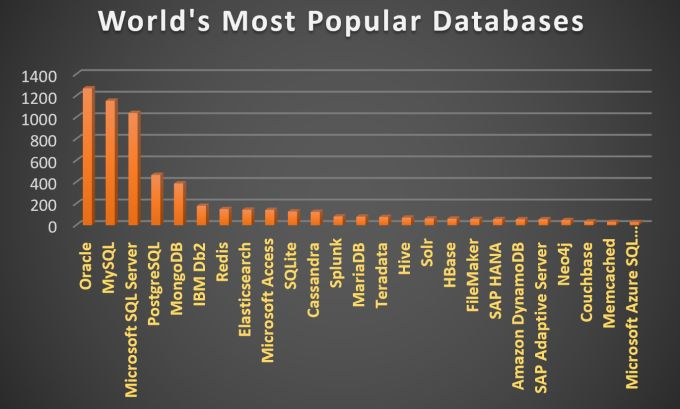
\includegraphics[width=\textwidth]{popular_databases.jpg}
	\caption{2019 - Most Popular Databases In The World}
	\label{fig:dbms}
\end{figure}
